% globecom_paper.tex — Master scaffold for IEEE GLOBECOM 2026 submission

\documentclass[conference]{IEEEtran}
\IEEEoverridecommandlockouts

% --- Packages (venue template order 
% \usepackage[linesnumbered,vlined,ruled]{algorithm2e}
% \usepackage{algorithmic}
\usepackage{adjustbox}
\usepackage{textcomp}
% \usepackage{xcolor}
\usepackage{subcaption} 
\usepackage[T1]{fontenc}
% ======

\usepackage{array}
\usepackage[table]{xcolor}
% \usepackage[draft=true]{hyperref}
% \usepackage{hyperref}
\usepackage{cite}
\usepackage{amsmath,amssymb,amsfonts}
\usepackage{graphicx}
\usepackage{textcomp}
\usepackage{booktabs} 
\usepackage{multirow} 
\usepackage{tikz}
\usetikzlibrary{arrows.meta,positioning}
% \usepackage{algorithm}
% \usepackage[ruled,vlined]{algorithm2e}
% \usepackage{algorithmic}
\usepackage{algorithm}
\usepackage[noend]{algpseudocode}
\usepackage{appendix}

\renewcommand{\dbltopfraction}{0.95}
\renewcommand{\topfraction}{0.95}
\renewcommand{\textfraction}{0.05}
\setcounter{dbltopnumber}{2}

\setlength{\columnsep}{0.21 in}
\def\BibTeX{{\rm B\kern-.05em{\sc i\kern-.025em b}\kern-.08em T\kern-.1667em\lower.7ex\hbox{E}\kern-.125emX}}

% \def\BibTeX{{\rm B\kern-.05em{\sc i\kern-.025em b}\kern-.08em
%     T\kern-.1667em\lower.7ex\hbox{E}\kern-.125emX}}



% ---------------------------------------------------------------
\begin{document}

\title{How Sharp Should the Swords Be? \\Stress-Testing Defenses Against RAG Knowledge Poisoning%
}

% --- Authors (venue template: ordinal superscripts; \textit{} for dept/org) ---
\author{
    \IEEEauthorblockN{
    Aquib Raza Raja\textsuperscript{\dag}, \textit{Student Member IEEE} \&
    % Asif Iqbal\textsuperscript{\S},\\
    Muhammad Naveed Aman\textsuperscript{\dag}, \textit{Senior Member IEEE} \\
    % and Biplab Sikdar\textsuperscript{\S}, \textit{Fellow IEEE} \\
    \textit{\textsuperscript{\dag}School of Computing, University of Nebraska-Lincoln, Lincoln, NE, USA.} \\
    % \textit{\textsuperscript{\S} Department of Electrical and Computer Engineering, National University of Singapore, Singapore.}
     Emails: \emph{araja2@huskers.unl.edu}; 
    % \emph{aiqbal@nus.edu.sg}; 
    \emph{naveed.aman@unl.edu}; 
    % \emph{bsikdar@nus.edu.sg}
    }
}

\maketitle

% --- Abstract ---
\begin{abstract}
% \input{sections/abstract}
\end{abstract}

\begin{IEEEkeywords}

\end{IEEEkeywords}

% ---------------------------------------------------------------
% SECTIONS
% ---------------------------------------------------------------

% --- I. Introduction ---
\section{Introduction}
% \input{sections/introduction}

% --- II. Threat Model and Attack Setting ---


\section{Threat Model and Attack Setting}
% \input{sections/threat_model}
\subsection{Hyoerparameter selection}
We set N=5 poisoned passages per target query to match the PoisonedRAG default setting. We evaluate k=5 and k=10 to separate two retrieval regimes. The k=5 setting corresponds to the PoisonedRAG default and represents a poison-saturated context where the number of retrieved passages equals the number of injected poisoned passages. The k=10 setting probes a mixed clean/poison regime where k > N, which PoisonedRAG’s own ablation identifies as the point where clean retrieved passages enter the context while poisoned passages are still usually retrieved. This mixed regime is particularly important for post-retrieval defenses such as RAGDefender and FilterRAG, because their filtering decisions depend on the composition of the retrieved top-k set.

% --- III. Defense Design ---
% \section{Proposed Inference-Time Defense}
% \input{sections/defense_design}

% --- IV. Baselines ---
\section{Baselines and Comparator Positioning}
\subsection{RAGDefender}
RAGDefender is effective under its stated assumptions, but our diagnostics show an important boundary condition: when top-k retrieval is fully saturated by poison, clean-anchor-based grouping cannot reliably rescue benign evidence because none is available.

RAGDefender explicitly assumes at least one benign passage is retrieved. Our diagnostics show that when this assumption is violated under full top-k retrieval saturation, its grouping and identification stages may fail or become ineffective. When k is expanded from 5 to 10, restoring clean context, RAGDefender substantially reduces ASR, but query-level estimator failures remain.

\subsubsection{Stage 2 Successful Case}
The following is a perfect case where all of the poisoned passages were removed as they clustered together, and none of the clean passages were affected.
\begin{figure}[H]
    \centering
    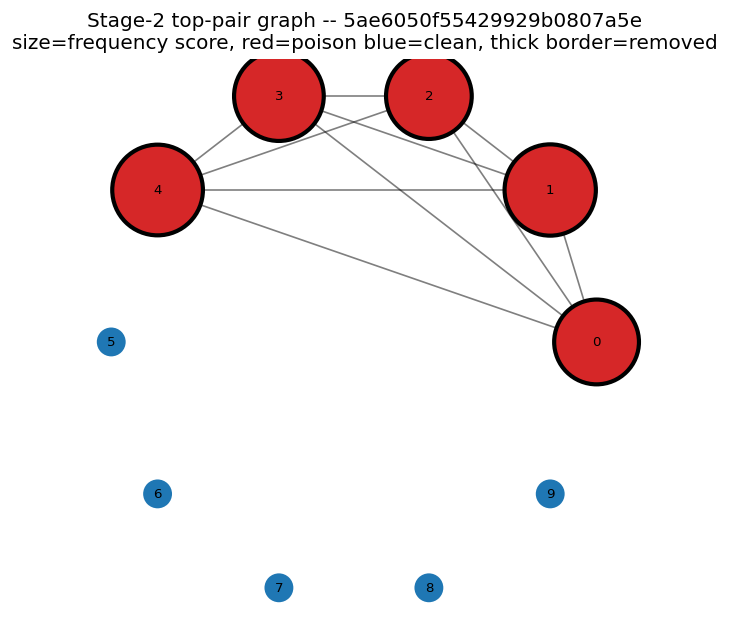
\includegraphics[width=0.5\linewidth]{figures/ragdef_case_success_807a5e_stage2_toppair.png}
    \caption{Caption}
    \label{fig:placeholder}
\end{figure}

\begin{figure}
    \centering
    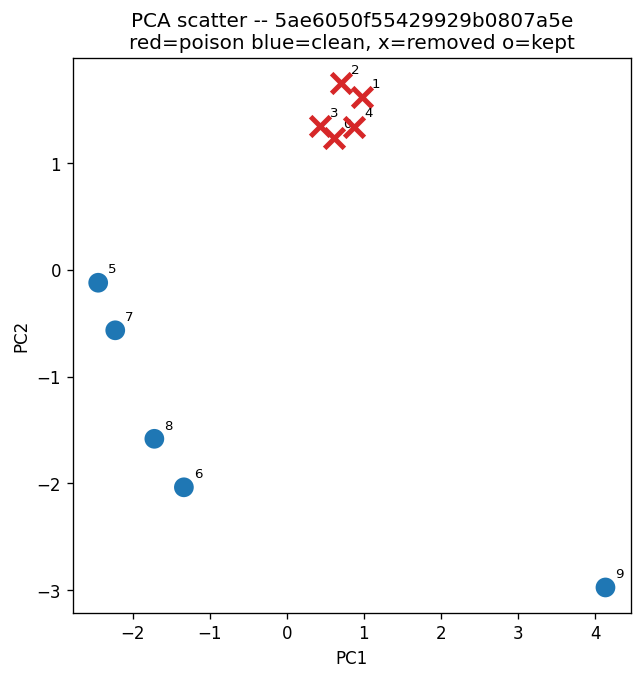
\includegraphics[width=0.5\linewidth]{figures/5ae6050f55429929b0807a5e_pca_scatter.png}
    \caption{Caption}
    \label{fig:placeholder}
\end{figure}

\subsubsection{Stage 2 Failure Case}
We instrument RAGDefender’s internal concentration and top-pair scoring pipeline and show that failures can arise when benign passages form a denser subgraph than adversarial passages. In such cases, the defense removes clean passages and leaves all poisoned passages intact.

RAGDefender correctly identifies the poison cluster, but Stage 1 overestimates $N_{adv}$, so Stage 2 removes extra clean passages.

\begin{figure}[H]
    \centering
    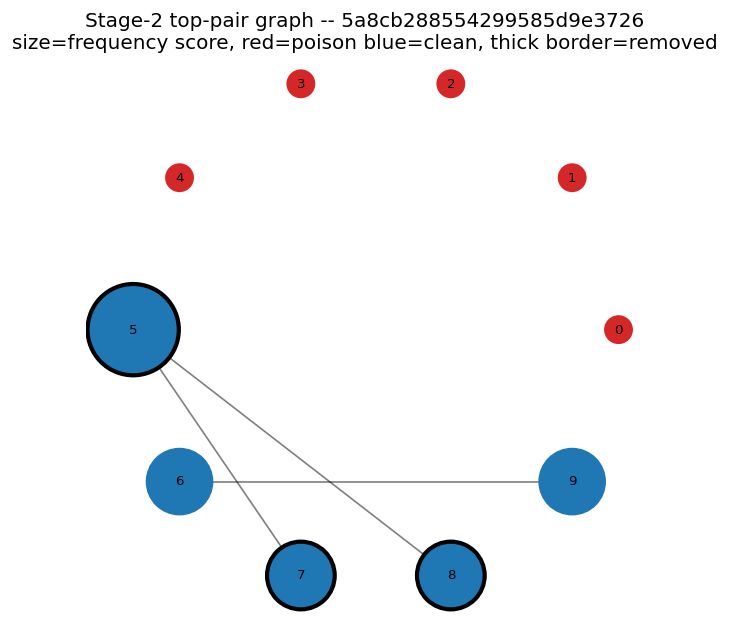
\includegraphics[width=0.5\linewidth]{figures/ragdef_case_failure_e3726_stage2_toppair.png}
    \caption{Caption}
    \label{fig:placeholder}
\end{figure}

\begin{figure}
    \centering
    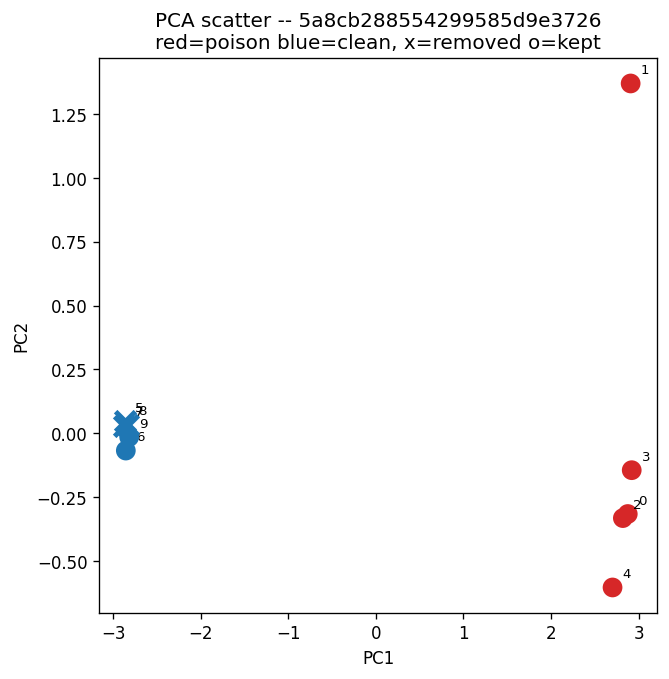
\includegraphics[width=0.5\linewidth]{figures/5a8cb288554299585d9e3726_pca_scatter.png}
    \caption{Caption}
    \label{fig:placeholder}
\end{figure}

The above case is a sample run where this defense technique lapsedl. but the following is where we carried out 'normalization' to elinminated clustering of posioned passage from a successful run in Fig 1 to a failure.

\subsubsection{Fragility}
If a defense relies on poison-poison cosine-density being higher than clean-clean or poison-clean density, then we can test how fragile that assumption is by applying representation-level normalization or distribution-matching operations that reduce the separability of poison-passage similarity statistics.

We use covariance alignment as an oracle diagnostic to test whether RAGDefender’s reliance on concentrated adversarial passage geometry is robust to distribution-normalized adversarial embeddings. We introduce an embedding-space normalization stress test for clustering-based RAG defenses. By matching the pairwise similarity distribution of adversarial passages to benign retrieved passages, we show that RAGDefender’s top-pair frequency heuristic is brittle to representation-level dispersion, motivating defenses that do not rely solely on adversarial passage density.


****success figure*****

We further approximate this oracle intervention using semantics-preserving passage rewrites that diversify adversarial evidence while preserving target-answer influence.

**multiple success case figures*

Across six originally successful HotpotQA k=10/N=5 RAGDefender cases, E1 clean-anchor oracle interpolation caused residual poisoned passages to survive in 22/24 query-strategy configurations. PP top-pair weakening preceded or coincided with residual-poison failure in all informative configurations, supporting the hypothesis that RAGDefender’s success depends on poisoned passages remaining the dominant dense top-pair subgraph.

\subsection{E1 causes MMD & CORAL variation?}
To verify that clean-anchor interpolation was not merely an arbitrary perturbation, we computed distribution-level distances between poisoned and clean embedding groups for every alpha step. Across 24 query-strategy configurations, both CORAL distance and RBF-MMD decreased monotonically as alpha decreased, indicating that the oracle intervention consistently moved poisoned embeddings toward the clean embedding distribution. However, top-pair poison-poison count was the most specific indicator of actual RAGDefender failure, consistent with RAGDefender’s Stage-2 reliance on dense pairwise similarity structure.

\subsection{CORAL impact}
CORAL is used as a covariance-alignment oracle: poisoned embeddings are treated as the source distribution and clean embeddings as the target distribution. MMD is used as a kernel mean-matching oracle objective over the same frozen embedding space. These are not text-space attacks or learned domain-adaptation models; they are formal embedding-space stress tests of RAGDefender’s similarity-based decision rule.

\subsection{Semantics-preserving textual adversarial attacks}
Will need when I move from embedding-only stress tests to real passage mutation. TextFooler, BERT-Attack, SemAttack, and TextAttack all support the general idea that text can be changed while preserving fluency/semantics and altering model behavior or embedding-space similarity. TextFooler emphasizes semantic preservation and grammaticality; BERT-Attack uses masked LM substitutions to generate fluent adversarial text; SemAttack explicitly uses different semantic spaces, including contextualized embedding spaces; TextAttack includes sentence-encoder cosine constraints such as SBERT/USE



\subsection{Filter-RAG}

\subsection{ML-Filter-RAG}

At $t=0.40$, ML-FilterRAG-top-$k$ reduces clean false positives from 78.1\% to 15.6\% relative to semantic threshold FilterRAG, while maintaining 94.9\% poison recall and a lower residual poison fraction.

\begin{table*}[!t]
\centering
\caption{HotpotQA 50-query held-out dry-run threshold sweep for ML-FilterRAG-top-$k$.
Evaluation covers 10 held-out query IDs, 20 $(q,k)$ records, 118 retrieved poisoned passages, and 32 retrieved clean passages.}
\label{tab:mlfilterrag_threshold_sweep}
\scriptsize
\setlength{\tabcolsep}{4pt}
\renewcommand{\arraystretch}{0.92}
\begin{tabular}{lccccc}
\toprule
Method / Threshold & Removed Poison & Removed Clean & Poison Recall & Clean FPR & Residual Poison \\
\midrule
FilterRAG semantic, $\epsilon=0.2$ & 116/118 & 25/32 & 0.9831 & 0.7813 & 0.2222 \\
\midrule
ML-FilterRAG, $t=0.10$ & 118/118 & 21/32 & 1.0000 & 0.6563 & 0.0000 \\
ML-FilterRAG, $t=0.30$ & 113/118 & 10/32 & 0.9576 & 0.3125 & 0.1852 \\
ML-FilterRAG, $t=0.35$ & 113/118 & 7/32  & 0.9576 & 0.2188 & \textbf{0.1667} \\
ML-FilterRAG, $t=0.40$ & 112/118 & 5/32  & 0.9492 & \textbf{0.1563} & 0.1818 \\
ML-FilterRAG, $t=0.50$ & 108/118 & 5/32  & 0.9153 & \textbf{0.1563} & 0.2703 \\
ML-FilterRAG, $t=0.70$ & 97/118  & 2/32  & 0.8220 & 0.0625 & 0.4118 \\
ML-FilterRAG, $t=0.90$ & 80/118  & 0/32  & 0.6780 & 0.0000 & 0.5429 \\
\bottomrule
\end{tabular}
\vspace{-0.5em}
\end{table*}

\subsubsection{ML-Filter-RAG Oracle Test}
At the selected operating threshold t=0.40, nearest-clean feature interpolation reduces poison recall from 94.9\% to 67.8\% at alpha=0.4, and below 50\% by alpha=0.2.

A held-out feature-space oracle stress test shows that ML-FilterRAG-top-k is sensitive to normalization of poisoned passages toward the clean feature distribution. At threshold t=0.40, nearest-clean interpolation reduces poison recall from 94.9\% at alpha=1.0 to 67.8\% at alpha=0.4, while increasing the residual poison fraction from 18.2\% to 58.5\%. This indicates that the learned classifier relies on separability in the four-dimensional feature space and can be weakened by feature-level distribution matching. This is an oracle feature-space test, not a text-realizable attack.

We further evaluate ML-FilterRAG-top-$k$ using a feature-space oracle stress test.  For each poisoned passage feature vector $z_{\mathrm{poison}}$, we construct $z'=\alpha z_{\mathrm{poison}}+(1-\alpha)z_{\mathrm{target}}$, where $z_{\mathrm{target}}$ is derived from clean-passage feature vectors.  The parameter $\alpha$ controls the intervention strength: $\alpha=1$ leaves the original poisoned features unchanged, while smaller $\alpha$ moves them toward clean-like feature statistics. This oracle does not rewrite passage text and therefore does not constitute a text-realizable attack; it tests whether the learned ML-FilterRAG decision boundary is fragile under clean-feature normalization.

% \input{sections/baselines}
\subsubsection{RobustRAG-KW}

\subsubsection{RobustRAG-KW Oracle Test}
In the 3-case full-retrieval pilot, RobustRAG-KW produced a different failure profile from RAGDefender, FilterRAG, and ML-FilterRAG. On the Ferocactus case, where low-overlap mutations weakened FilterRAG and ML-FilterRAG, RobustRAG-KW returned the correct answer. On the Gibson case, RobustRAG-KW also failed, showing that answer aggregation is not a universal defense. On the Schmeichel case, RobustRAG-KW abstained, suggesting a safety–coverage tradeoff.

% --- V. Experimental Setup ---
\section{Experimental Setup}
% \input{sections/setup}



% --- VI. Metrics and Evaluation Protocol ---
\section{Metrics and Evaluation Protocol}
% \input{sections/metrics}

% --- VII. Results ---
\section{Results}
% \input{sections/results}

\section{Limitations}
% \input{sections/limitations}

% --- IX. Conclusion ---
\section{Conclusion}
% \input{sections/conclusion}

% ---------------------------------------------------------------
% \section*{Acknowledgment}

% ---------------------------------------------------------------
% Bibliography — use external .bib file with IEEEtran style
\bibliographystyle{IEEEtran}
\bibliography{references}

\clearpage

\begin{appendices}
\subsection{RAGDefender Multi-Hop Filtering}
\label{subsec:ragdefender}

RAGDefender is a post-retrieval filtering defense that attempts to
identify poisoned passages from their pairwise similarity structure
before the retrieved context is provided to the generator
\cite{kim2025ragdefender}. For the HotpotQA multi-hop setting, the
defense operates in two stages. The first stage estimates the number of
adversarial passages in the retrieved set, while the second stage
identifies and removes that number of passages.

Let
\begin{equation}
\mathcal{D}=\{d_1,d_2,\ldots,d_k\}
\end{equation}
denote the top-$k$ retrieved passages for a query. Each passage $d_i$ is
encoded using the \texttt{paraphrase-MiniLM-L6-v2} sentence encoder,
producing an embedding $\mathbf{z}_i$. The defense constructs the
pairwise cosine-similarity matrix
\begin{equation}
S_{ij}
=
\cos(\mathbf{z}_i,\mathbf{z}_j)
=
\frac{\mathbf{z}_i^{\top}\mathbf{z}_j}
{\|\mathbf{z}_i\|_2\|\mathbf{z}_j\|_2},
\qquad 1\leq i,j\leq k.
\label{eq:ragdefender_cosine}
\end{equation}

\subsubsection{Stage 1: Adversarial-Count Estimation}

For each passage, RAGDefender calculates the mean and median of its
similarities to all retrieved passages:
\begin{align}
\mu_i
&=
\frac{1}{k}\sum_{j=1}^{k}S_{ij},
\label{eq:passage_mean_similarity}\\
m_i
&=
\operatorname{median}_{1\leq j\leq k} S_{ij}.
\label{eq:passage_median_similarity}
\end{align}
In the evaluated implementation, these statistics include the diagonal
self-similarity term $S_{ii}=1$.

The passage-level statistics are summarized by a global mean
\begin{equation}
\bar{\mu}
=
\frac{1}{k}\sum_{i=1}^{k}\mu_i
\label{eq:global_mean_similarity}
\end{equation}
and a global median
\begin{equation}
\widetilde{m}
=
\operatorname{median}_{1\leq i\leq k} m_i.
\label{eq:global_median_similarity}
\end{equation}

RAGDefender then evaluates two concentration tests for each passage.
The mean-based indicator is
\begin{equation}
a_i
=
\mathbb{I}\!\left[\mu_i>\bar{\mu}\right],
\label{eq:mean_indicator}
\end{equation}
where $\mathbb{I}[\cdot]$ is the indicator function. The threshold for
the median-based test is the midpoint between the global mean and
global median:
\begin{equation}
\tau_m
=
\frac{\bar{\mu}+\widetilde{m}}{2}.
\label{eq:median_threshold}
\end{equation}
The corresponding median-based indicator is
\begin{equation}
b_i
=
\mathbb{I}\!\left[m_i>\tau_m\right].
\label{eq:median_indicator}
\end{equation}

The two indicators are combined using a logical OR:
\begin{equation}
f_i
=
a_i\lor b_i.
\label{eq:or_flag}
\end{equation}
Thus, a passage is included in the initially concentrated group if
either its mean similarity exceeds the global mean or its median
similarity exceeds the median threshold. Let
\begin{equation}
c
=
\sum_{i=1}^{k}f_i
\label{eq:raw_flag_count}
\end{equation}
denote the number of passages satisfying this OR rule.

The final adversarial-count estimate includes a flip branch:
\begin{equation}
\widehat{N}_{\mathrm{adv}}
=
\begin{cases}
c,
&
c>0\ \land\ \bar{\mu}<\widetilde{m},\\[3pt]
k-c,
&
\text{otherwise}.
\end{cases}
\label{eq:adv_count_estimate}
\end{equation}
Consequently, the defense does not always interpret the passages
satisfying the concentration tests as adversarial. Depending on the
relationship between $\bar{\mu}$ and $\widetilde{m}$, it may instead
treat the complementary group as adversarial. Stage~1 returns only the
estimated count $\widehat{N}_{\mathrm{adv}}$; its passage-level flags
are not directly used as the final removal decision.

\subsubsection{Stage 2: Pair-Frequency Identification}

Stage~2 uses $\widehat{N}_{\mathrm{adv}}$ to determine how many
high-similarity passage pairs should be examined. If
$\widehat{N}_{\mathrm{adv}}$ adversarial passages form a dense group,
they induce
\begin{equation}
L
=
\max\left(
1,
\binom{\widehat{N}_{\mathrm{adv}}}{2}
\right)
=
\max\left(
1,
\frac{\widehat{N}_{\mathrm{adv}}
(\widehat{N}_{\mathrm{adv}}-1)}{2}
\right)
\label{eq:number_selected_pairs}
\end{equation}
candidate within-group pairs.

The defense enumerates all non-self pairs
\begin{equation}
\mathcal{P}
=
\{(i,j,S_{ij}) : 1\leq i<j\leq k\}
\end{equation}
and ranks them in descending order of $S_{ij}$. Let
$\mathcal{P}_L$ denote the $L$ most similar pairs.

Each selected pair contributes a signed squared-similarity weight
\begin{equation}
w_{ij}
=
\operatorname{sign}(S_{ij})|S_{ij}|^2.
\label{eq:signed_squared_similarity}
\end{equation}
For the predominantly positive cosine similarities observed among
retrieved passages, this reduces to $w_{ij}=S_{ij}^{2}$. Squaring the
similarity gives greater weight to the most concentrated passage pairs.

The suspicion score assigned to passage $d_i$ is
\begin{equation}
r_i
=
\sum_{(u,v,S_{uv})\in\mathcal{P}_L}
w_{uv}
\left(
\mathbb{I}[i=u]+\mathbb{I}[i=v]
\right).
\label{eq:passage_frequency_score}
\end{equation}
A passage therefore receives a high score when it participates
frequently in the selected pair set and when the corresponding pairwise
similarities are large. The defense ranks passages by $r_i$ and removes
the $\widehat{N}_{\mathrm{adv}}$ highest-scoring passages:
\begin{equation}
\mathcal{D}_{\mathrm{remove}}
=
\operatorname{TopK}
\left(
\{r_i\}_{i=1}^{k},
\widehat{N}_{\mathrm{adv}}
\right).
\label{eq:removed_passages}
\end{equation}

The filtered context supplied to the generator is
\begin{equation}
\mathcal{D}_{\mathrm{filtered}}
=
\mathcal{D}\setminus\mathcal{D}_{\mathrm{remove}}.
\label{eq:filtered_context}
\end{equation}

The procedure relies on the assumption that poisoned passages form the
densest high-similarity subgraph among the retrieved passages. When the
top-$L$ pairs are predominantly poison--poison pairs, the poisoned
passages accumulate the largest scores and are removed. Conversely, the
defense can remove benign passages when clean passages form a denser
subgraph, or when poison--clean similarities dominate the selected pair
set. The latter cases represent failures of the relative-concentration
assumption rather than failures of the pair-scoring implementation.

Our diagnostic implementation reproduces the baseline calculations
without modifying the filtering behavior. It records the passage-level
means and medians, global thresholds, OR flags, flip-branch decision,
selected Stage-2 pairs, accumulated frequency scores, and final removal
indices. These quantities permit direct analysis of whether a defense
outcome is caused by adversarial-count estimation in Stage~1 or by
incorrect top-pair composition in Stage~2.
\end{appendices}

\end{document}
